
% ----------------------------------------------------------------------
% Set the document class
% ----------------------------------------------------------------------
\documentclass[12pt	]{article}
\usepackage{multirow}
\usepackage{matlab-prettifier}



% ----------------------------------------------------------------------
% Define external packages, language, margins, fonts, new commands 
% and colors
% ----------------------------------------------------------------------
\usepackage[utf8]{inputenc} % Codification
\usepackage[english]{babel} % Writing idiom

\usepackage[export]{adjustbox} % Align images
\usepackage{amsmath} % Extra commands for math mode
\usepackage{amssymb} % Mathematical symbols
\usepackage{anysize} % Personalize margins
    \marginsize{2cm}{2cm}{2cm}{2cm} % {left}{right}{above}{below}
    
    

\usepackage{appendix} % Appendices
\usepackage{cancel} % Expression cancellation
\usepackage{caption} % Captions
\usepackage{listings}
\usepackage{xcolor}



    \DeclareCaptionFont{newfont}{\fontfamily{cmss}\selectfont}
    \captionsetup{labelfont={bf, newfont}}
\usepackage{cite} % Citations, like [1 - 3]
\usepackage{color} % Text coloring
\usepackage{fancyhdr} % Head note and footnote
    \pagestyle{fancy}
    \fancyhf{}
    \fancyhead[L]{\footnotesize \fontfamily{cmss}\selectfont Dependable System Design} % Left of Head note
    \fancyhead[R]{\footnotesize \fontfamily{cmss}\selectfont CE5407} % Right of Head note
    \fancyfoot[L]{\footnotesize \fontfamily{cmss}\selectfont CE Dep.} % Left of Footnote
    \fancyfoot[C]{\thepage} % Center of Footnote
    \fancyfoot[R]{\footnotesize \fontfamily{cmss}\selectfont AUT} % Right of Footnote
    \renewcommand{\footrulewidth}{0.4pt} % Footnote rule
\usepackage{float} % Utilization of [H] in figures
\usepackage{graphicx} % Figures in LaTeX
\usepackage[colorlinks = true, plainpages = true, linkcolor = blue, urlcolor = blue, citecolor = blue, anchorcolor = blue]{hyperref}
\usepackage{indentfirst} % First paragraph
\usepackage[super]{nth} % Superscripts
\usepackage{siunitx} % SI units
\usepackage{subcaption} % Subfigures
\usepackage{titlesec} % Font
    \titleformat{\section}{\fontfamily{cmss}\selectfont\Large\bfseries}{\thesection}{1em}{}
    \titleformat{\subsection}{\fontfamily{cmss}\selectfont\large\bfseries}{\thesubsection}{1em}{}
    \titleformat{\subsubsection}{\fontfamily{cmss}\selectfont\normalsize\bfseries}{\thesubsubsection}{1em}{}
    \fancyfoot[C]{\fontfamily{cmss}\selectfont\thepage}

% Random text (not needed)
\usepackage{lipsum}
\usepackage{duckuments}

% New and re-newcommands
\newcommand{\sen}{\operatorname{\sen}} % Sine function definition
\newcommand{\HRule}{\rule{\linewidth}{0.5mm}} % Specific rule definition
\renewcommand{\appendixpagename}{\LARGE \fontfamily{cmss}\selectfont Appendices}

% Colors
\definecolor{istblue}{RGB}{3, 171, 230}
\definecolor{dkgreen}{rgb}{0,0.6,0}
\definecolor{gray}{rgb}{0.5,0.5,0.5}

% Image path
\graphicspath{ {./Images/} }

\usepackage[most]{tcolorbox}



% Some definitions to use color
% Default fixed font does not support bold face
\DeclareFixedFont{\ttb}{T1}{txtt}{bx}{n}{9} % for bold
\DeclareFixedFont{\ttm}{T1}{txtt}{m}{n}{9}  % for normal

% Custom colors
\usepackage{color}
\definecolor{deepblue}{rgb}{0,0,0.5}
\definecolor{deepred}{rgb}{0.6,0,0}
\definecolor{deepgreen}{rgb}{0,0.5,0}

\usepackage{listings}

% Define a custom style for Bash

\lstdefinestyle{bashstyle}{
	language=bash,
	basicstyle=\ttfamily\small,         % Font style for the code
	keywordstyle=\color{blue}\bfseries, % Style for keywords
	stringstyle=\color{red},            % Style for strings
	commentstyle=\color{deepgreen},     % Dark green for comments
	showstringspaces=false,             % Do not show spaces in strings
	numbers=left,                       % Line numbers on the left
	numberstyle=\tiny\color{gray},      % Style for line numbers
	numbersep=5pt,                      % Space between line numbers and code
	frame=single,                       % Add a border around the code
	rulecolor=\color{black},            % Border color
	breaklines=true,                    % Allow line breaks
	escapeinside={(*@}{@*)},            % Escape inside commands for adding symbols
	prebreak=\mbox{\textcolor{blue}{\$}\hspace{0.5em}}, % Prebreak adds blue $
}

\lstset{style=bashstyle}


%%%%%%%%%%%%%%%%%%%%%%%%%%%%%%%%%%%%%%%%%% Solution box setting %%%%%%%%%%%%%%%%%%%%%%%%%%%%%%%%%%%%%%%%%%
\newtcbtheorem{Problem}{\bfseries Problem}{enhanced,drop shadow={black!50!white},
	coltitle=black,
	top=0.3in,
	attach boxed title to top left=
	{xshift=1.5em,yshift=-\tcboxedtitleheight/2},
	boxed title style={size=small,colback=pink}
}{summary}

\newtcolorbox[auto counter]{summary}[1][]{title={\bfseries Problem~\thetcbcounter},enhanced,drop shadow={black!50!white},
	coltitle=black,
	top=0.3in,
	attach boxed title to top left=
	{xshift=1.5em,yshift=-\tcboxedtitleheight/2},
	boxed title style={size=small,colback=pink},#1}
	
%%%%%%%%%%%%%%%%%%%%%%%%%%%%%%%%%%%%%%%%%%%%%%%%%%%%%%%%%%%%%%%%%%%%%%%%
%                                 Document                             %
%%%%%%%%%%%%%%%%%%%%%%%%%%%%%%%%%%%%%%%%%%%%%%%%%%%%%%%%%%%%%%%%%%%%%%%%
\begin{document}

% ----------------------------------------------------------------------
% Cover
% ----------------------------------------------------------------------
\begin{center}
    \begin{figure}
        \vspace{-1.0cm}
        \centering
        
\includegraphics[scale = 0.35]{Images/AUT_logo.png} % IST logo
    \end{figure}
    \mbox{}\\[2.0cm]
    \textsc{\Huge \textbf{Dependable System Design}}\\[1.0cm]
    \textsc{\LARGE Instructor: \href{https://scholar.google.com/citations?user=ZA9rRWAAAAAJ&hl=en}{\textcolor{black}{Prof. Hamid R. Zarandi}}}\\[2.5cm]
    \textsc{\LARGE Amirkabir University of Technology} \\%\\[1.0cm]
    \textsc{(Tehran polytechnic)}
    \HRule\\[0.4cm]
    {\large \bf {\fontfamily{cmss}\selectfont RBD Calculator} }\\[0.2cm]
    \HRule\\[1.5cm]
\end{center}

\begin{flushleft}
    \textbf{\fontfamily{cmss}\selectfont Authors:}
\end{flushleft}

\begin{center}
    \begin{minipage}{0.5\textwidth}
        \begin{flushleft}
            \href{https://rezaadinepour.github.io/}{\textcolor{black}{Reza Adinepour}}\\
        \end{flushleft}
    \end{minipage}%
    \begin{minipage}{0.5\textwidth}
        \begin{flushright}
            \href{mailto:adinepour@aut.ac.ir}{\texttt{adinepour@aut.ac.ir}}
        \end{flushright}
    \end{minipage}
\end{center}

\vspace{1em}

    
\begin{center}
    \bigskip \bigskip \bigskip \bigskip
    \large \bf \fontfamily{cmss}\selectfont Fall 2024
\end{center}

\thispagestyle{empty}

\setcounter{page}{0}

\newpage

% ----------------------------------------------------------------------
% Contents
% ----------------------------------------------------------------------
\tableofcontents

\newpage

% ----------------------------------------------------------------------
% Body
% ----------------------------------------------------------------------

% ------------------Section 1--------------------

%\begin{figure}[h]
%	\centering
%	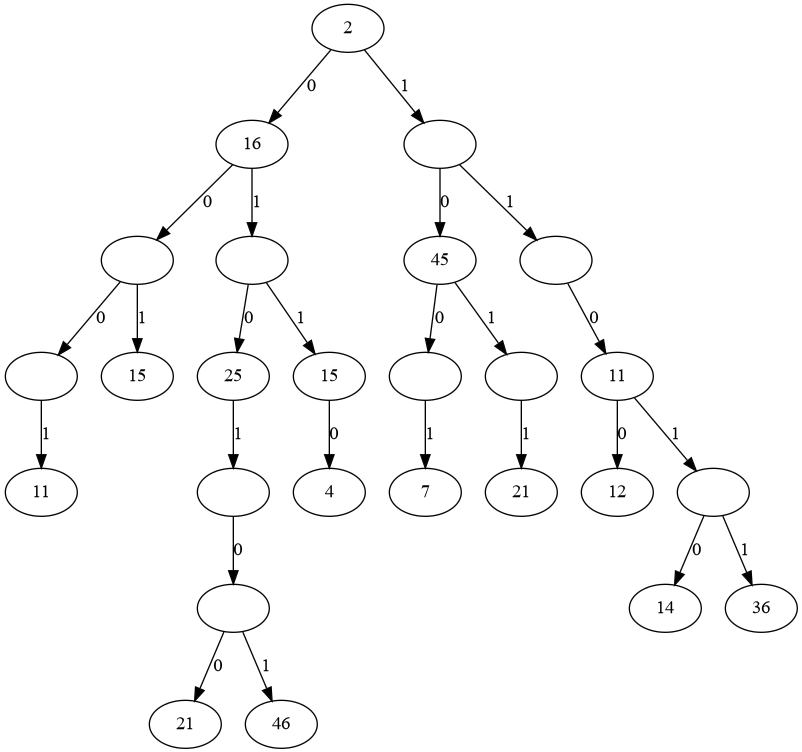
\includegraphics[width=0.8\textwidth]{Images/img6.png}
%	\caption{Overview of cyber physical systems.}
%	\label{fig:Overview of cyber physical systems}
%\end{figure}


\section{Introduction}
The Reliability Block Diagram (RBD) method is a graphical and analytical approach used to model and evaluate the reliability of systems. It represents a system as a combination of interconnected blocks, each corresponding to a system component or subsystem, with the connections illustrating their functional relationships. By analyzing the configuration of these blocks—whether in series, parallel, or complex hybrid structures—engineers can predict the overall system reliability, identify weak points, and optimize designs to enhance performance. The RBD method is widely used in industries like aerospace, automotive, electronics, and manufacturing, where reliability is critical. Its flexibility allows for the modeling of simple systems as well as complex, interdependent systems with varying failure modes and repair strategies.



\section{Definition}
The Reliability Block Diagram (RBD) method involves calculating the reliability of a system based on the arrangement of its components. The total reliability depends on the configuration of these components—whether in series, parallel, or a combination. Below are the key formulas used in RBD analysis:

\subsection{Series Configuration}
In a series configuration, the failure of any single component leads to the failure of the entire system. The total reliability of a system with \(n\) components in series is given by:
\[
R_{\text{total}}(t) = \prod_{i=1}^{n} R_i(t)
\]



\subsection{Parallel Configuration}
In a parallel configuration, the system functions as long as at least one component remains operational. The total reliability of a system with \(n\) components in parallel is expressed as:
\[
R_{\text{total}}(t) = 1 - \prod_{i=1}^{n} \big(1 - R_i(t)\big)
\]


\subsection{$m-of-n$ Configuration}
An \(m\)-of-\(n\) configuration means the system operates if at least \(m\) out of \(n\) components are functioning. The total reliability of the system is calculated using the binomial distribution:

\[
R_{\text{total}}(t) = R_{m\text{-of-}n}(t) = \sum_{i=m}^{n} \binom{n}{i} R^i(t) \big(1 - R(t)\big)^{n-i}
\]




\section{Implementation}
We designed this project using two models:
\begin{enumerate}
	\item Standard Design: A conventional approach.
	\item GUI Design: A visual and interactive approach.
\end{enumerate}

The details of both models will be explained below.




\subsection{Standard Design}
In this section, by running the \texttt{main.py} code, you can input your model in the following format:

\begin{center}
	\texttt{Name of model-Start node-End node-Reliability}
\end{center}

For example, if you want to describe a system consisting of two subsystems in series and one parallel subsystem connected to the previous two (as shown in "Fig. \ref{fig:Example System}"),

\begin{figure}[h]
	\centering
	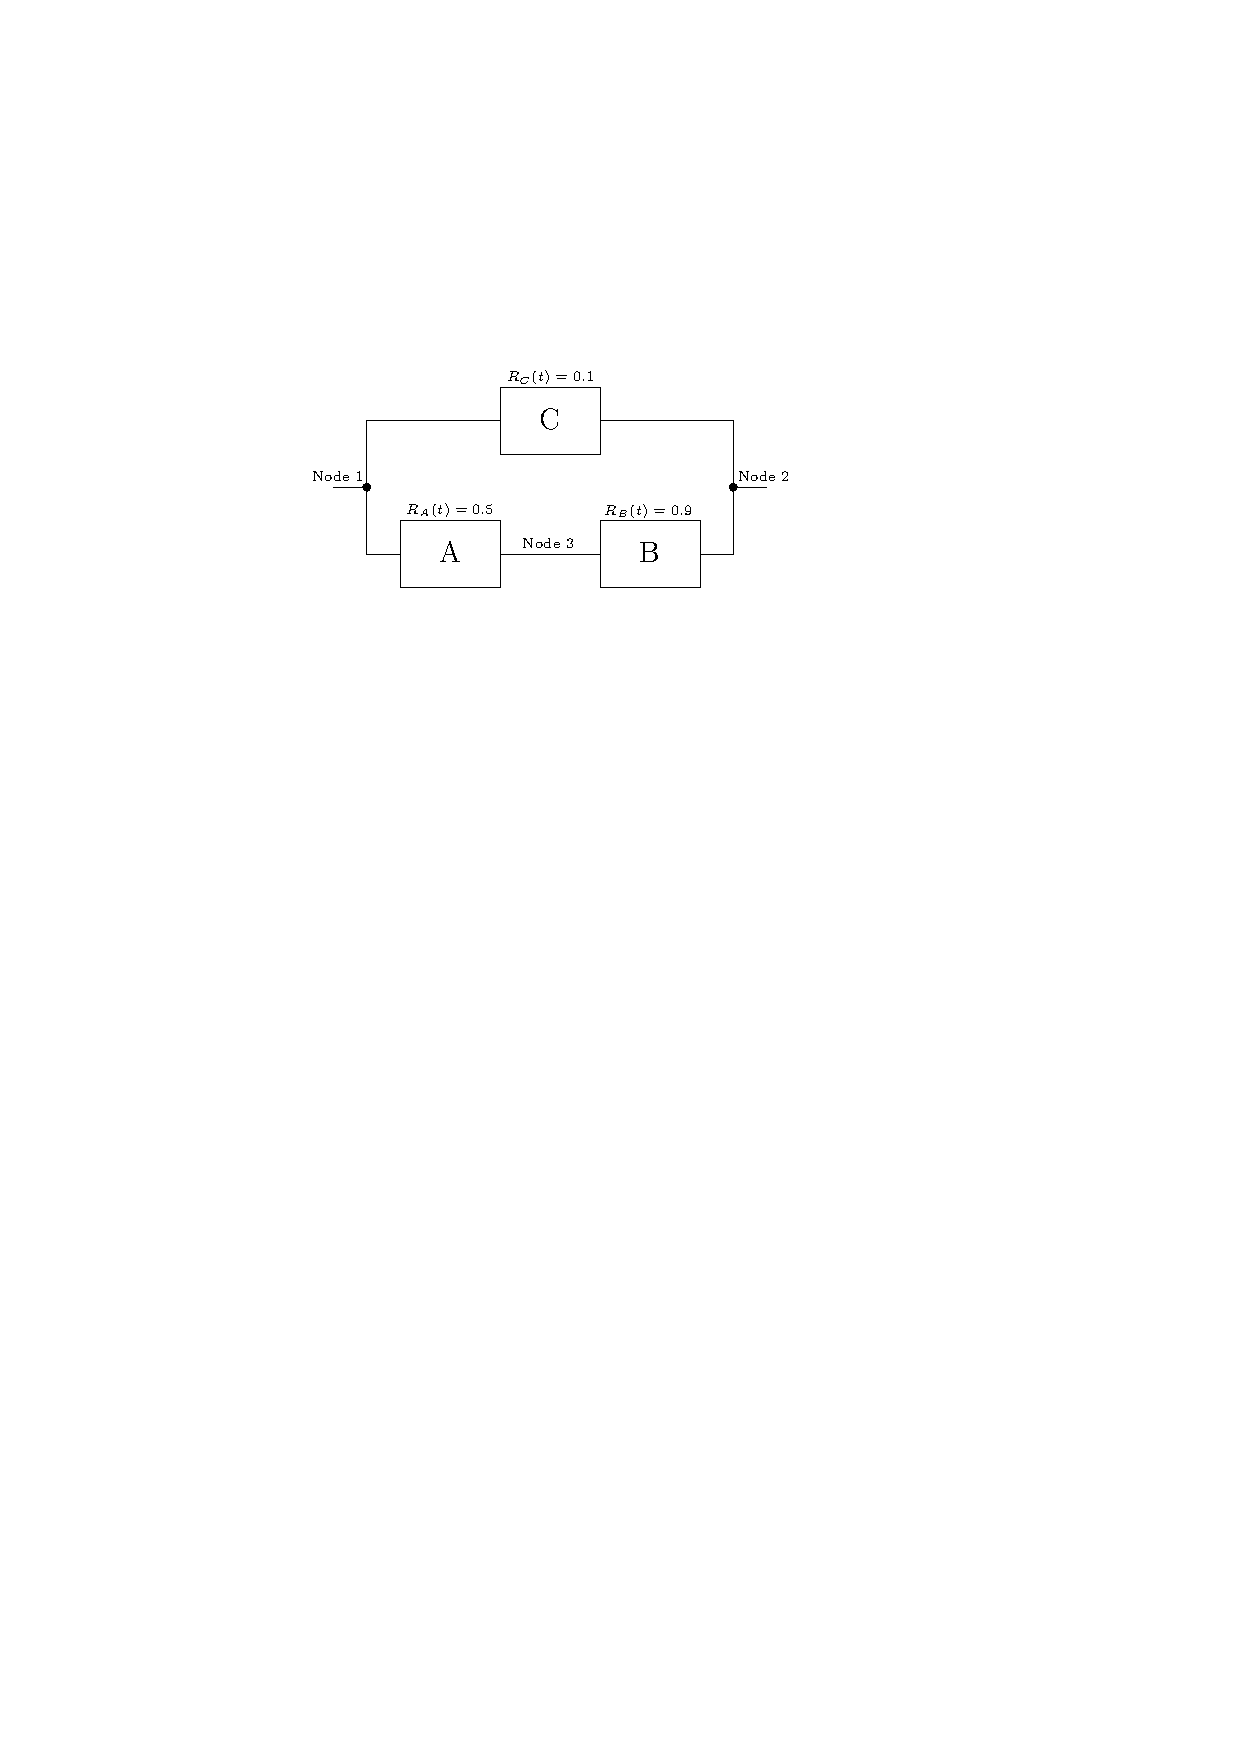
\includegraphics[width=0.6\textwidth]{Images/img1.pdf}
	\caption{Example System}
	\label{fig:Example System}
\end{figure}


you can proceed as follows:

\begin{center}
	\texttt{A-1-3-0.5, B-3-2-0.9, C-1-2-0.1}
\end{center}





\subsection{GUI Design}
In the web application developed using \texttt{NodeJS}, the server can be run as follows:

\subsubsection{Install Dependencies}
First, install the required dependencies as follows:


\begin{lstlisting}
# For Ubuntu/Debian:

(*@\textcolor{blue}{\$}@*) curl -fsSL https://deb.nodesource.com/setup_lts.x | sudo -E bash -
(*@\textcolor{blue}{\$}@*) sudo apt-get install -y nodejs

# For macOS (using Homebrew):
(*@\textcolor{blue}{\$}@*) brew install node

# For Windows:
# Download and run the installer from https://nodejs.org/en/download/
\end{lstlisting}


\subsubsection{Verify Installation}
\begin{lstlisting}
(*@\textcolor{blue}{\$}@*) node --version
(*@\textcolor{blue}{\$}@*) npm --version
\end{lstlisting}



\subsection{Run Application}
After installing all the dependencies, you can prepare the server to run using the following commands:

\begin{lstlisting}
(*@\textcolor{blue}{\$}@*) npm install
(*@\textcolor{blue}{\$}@*) npm run dev
\end{lstlisting}

The application should now be running as bellow! You can access it at \texttt{http://localhost:5173} (or whatever port Vite assigns).


\begin{figure}[h]
	\centering
	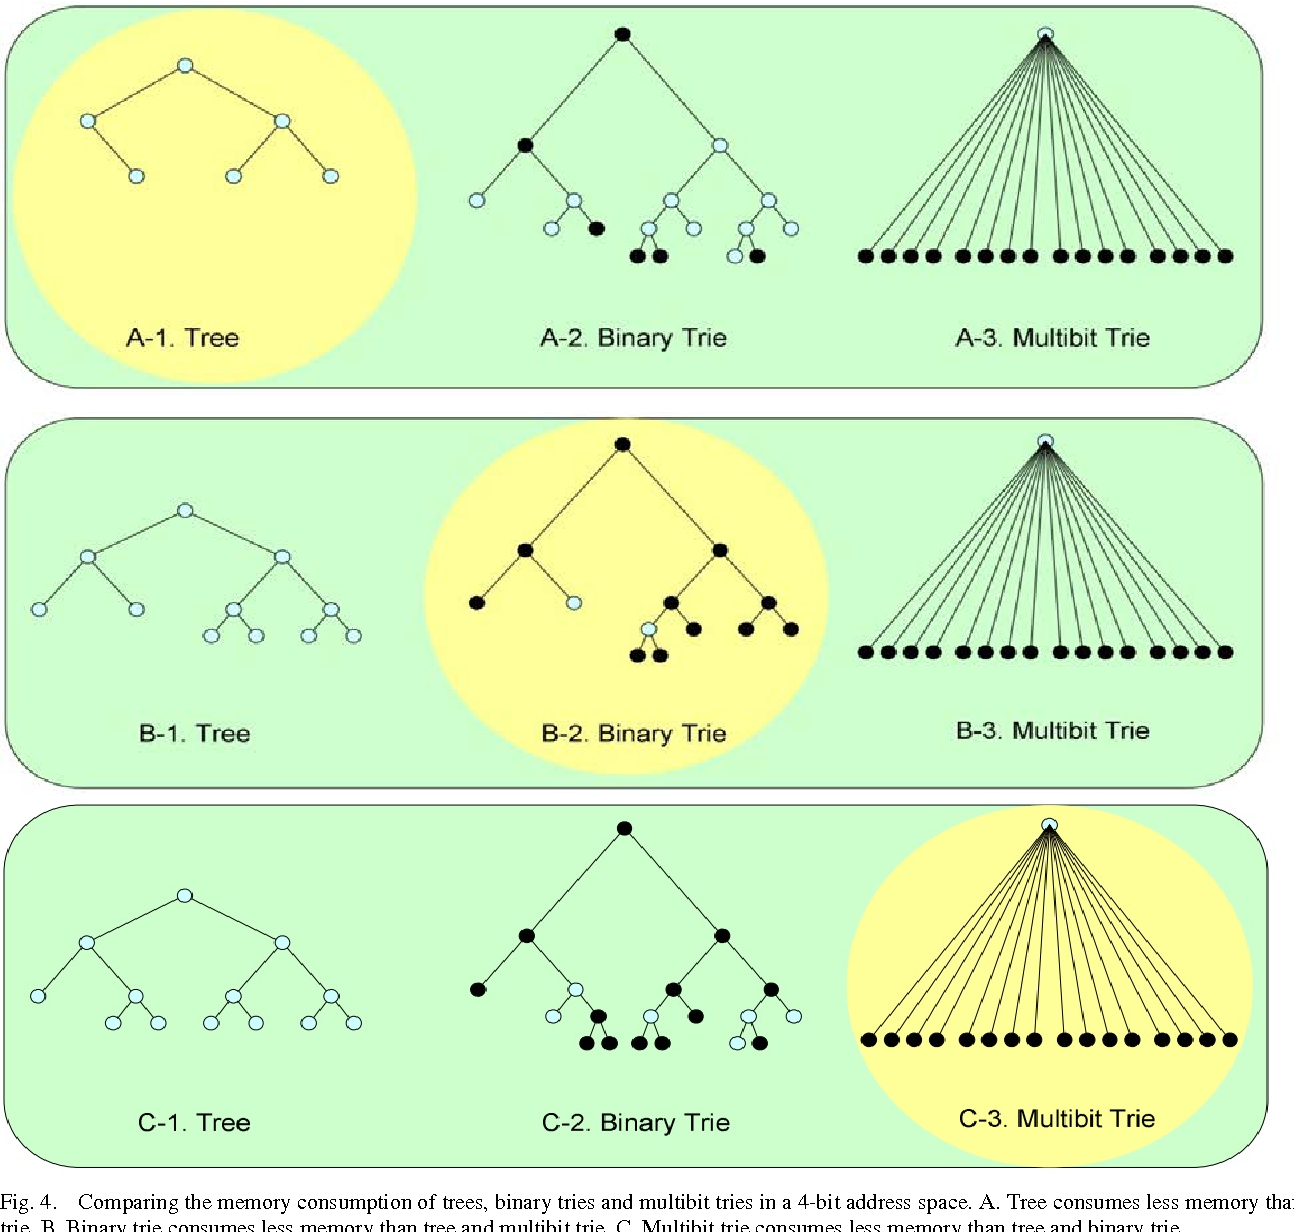
\includegraphics[width=0.65\textwidth]{Images/img2.png}
	\caption{Web Application Overview}
	\label{fig:WebApp}
\end{figure}

In this App, the inputs are entered in the same way as in the previous case.



\section{Evaluation}
To test the functionality of the developed program, several models are calculated theoretically, and the results are then compared with the outputs of the program.

\subsection{model 1}
We solve the model presented in Figure 1 theoretically.


The system configuration is as follows:
\begin{itemize}
	\item Subsystems $A$ and $B$ form a series path from node 1 to node 3 to node 2.
	\item Subsystem $C$ is in parallel with the series combination of $A$ and $B$, connecting node 1 directly to node 2.
\end{itemize}


\paragraph{Step 1: Series Combination of $A$ and $B$}

For the series combination of $A$ and $B$, the reliability is calculated as:
\[
R_{\text{series}} = R_A \cdot R_B
\]
Substituting $R_A = 0.5$ and $R_B = 0.9$:
\[
R_{\text{series}} = 0.5 \cdot 0.9 = 0.45
\]

This represents the reliability of the path $1 \to 3 \to 2$.


\paragraph{Step 2: Parallel Combination of $R_{\text{series}}$ and $C$}

The reliability of the parallel system, consisting of $R_{\text{series}}$ and $R_C$, is given by:
\[
R_{\text{parallel}} = 1 - \left[(1 - R_{\text{series}}) \cdot (1 - R_C)\right]
\]
Substituting $R_{\text{series}} = 0.45$ and $R_C = 0.1$:
\[
R_{\text{parallel}} = 1 - \left[(1 - 0.45) \cdot (1 - 0.1)\right]
\]
\[
R_{\text{parallel}} = 1 - \left[0.55 \cdot 0.9\right]
\]
\[
R_{\text{parallel}} = 1 - 0.495 = 0.505
\]


\paragraph{Step 3: Final Answer}

The total reliability of the system is approximately:
\[
\boxed{0.505}
\]


If we provide the same input to the application, the output will match the results of our analysis.

\newpage

\begin{figure}[h]
	\centering
	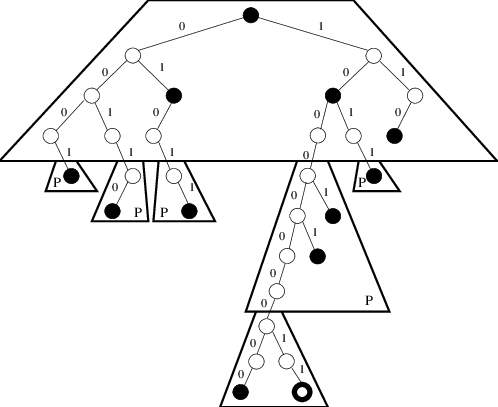
\includegraphics[width=0.45\textwidth]{Images/img3.png}
	\caption{Test of Model 1}
	\label{fig:Test of Model 1}
\end{figure}



\subsection{model 2}
If our model is as shown in the following figure:

\begin{figure}[h]
	\centering
	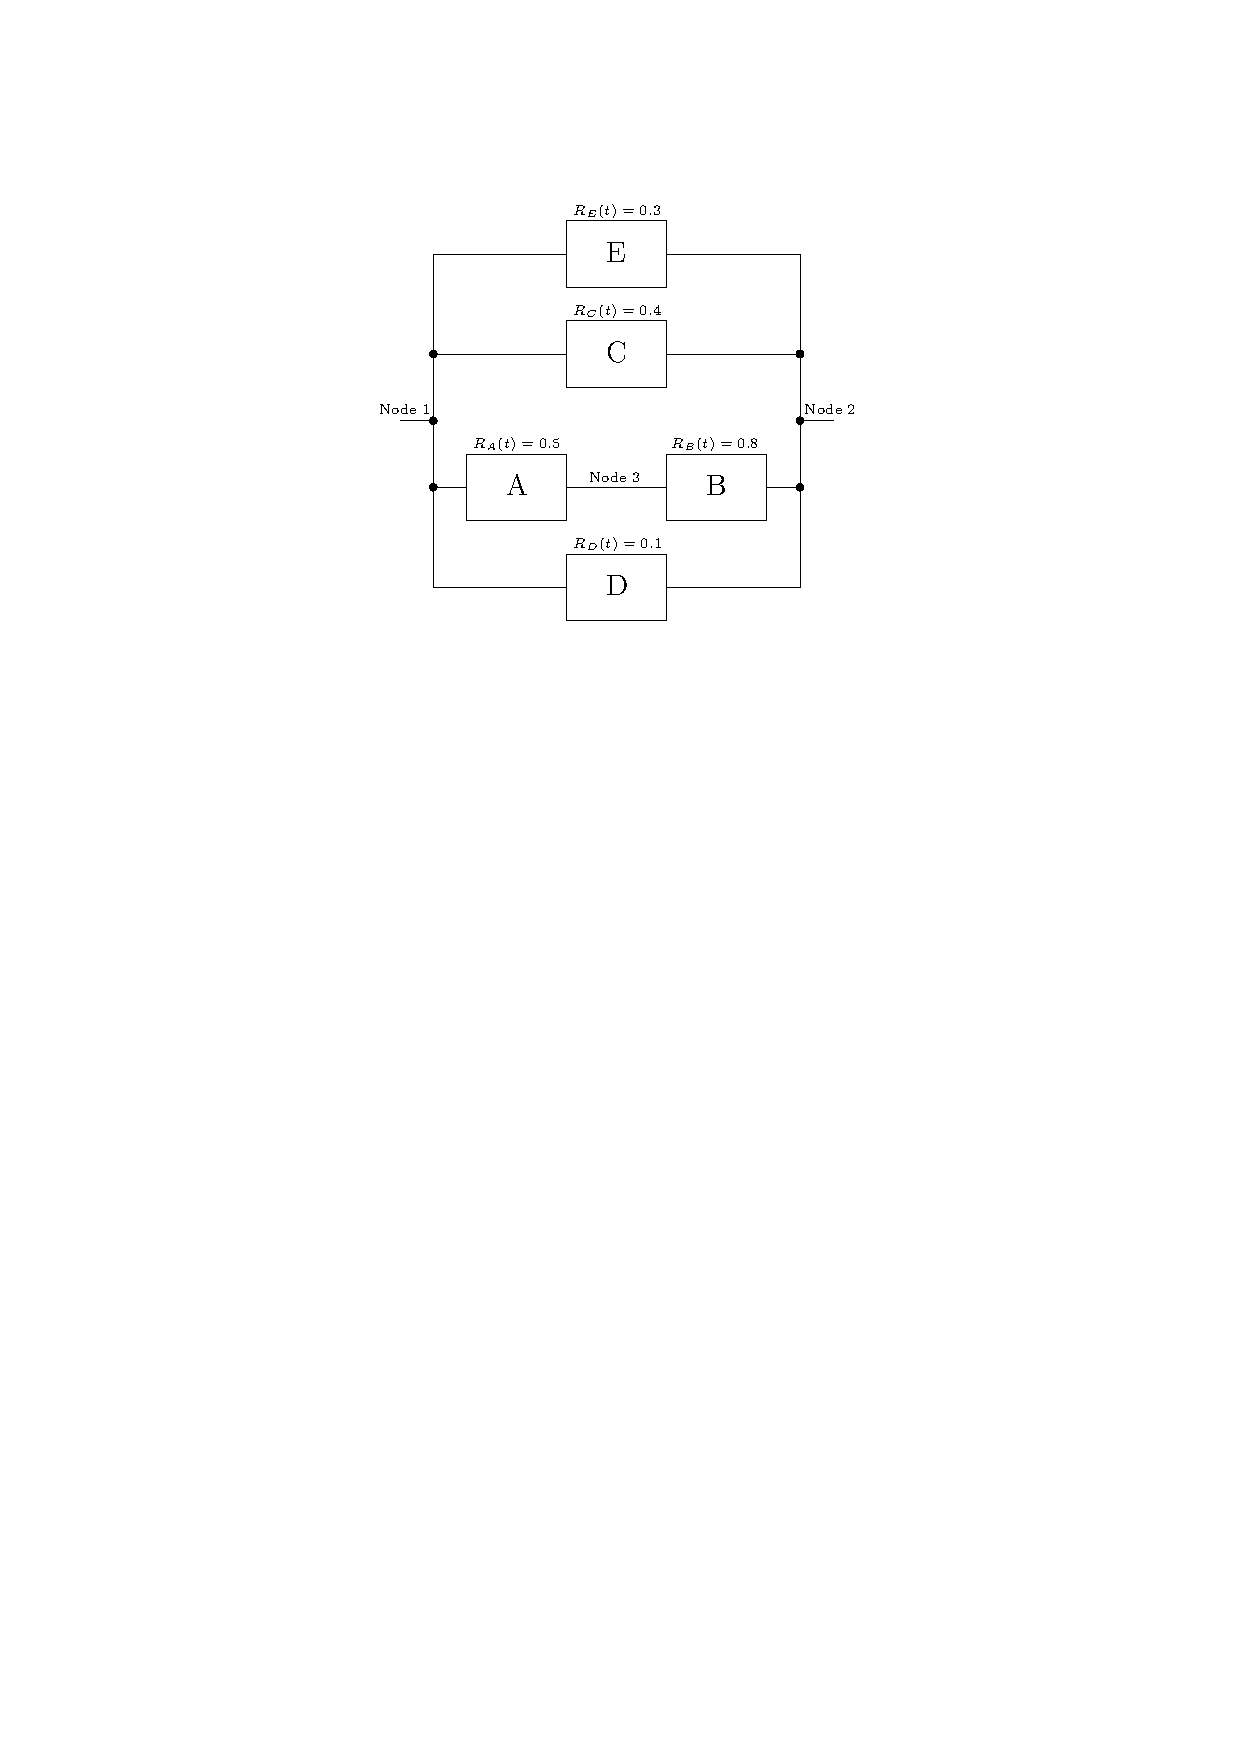
\includegraphics[width=0.45\textwidth]{Images/img3.pdf}
	\caption{Model 2}
	\label{fig:Model 2}
\end{figure}

It can be theoretically solved as follows:

\paragraph{Problem Setup}
We are given the following subsystems:
\begin{itemize}
	\item $A-1-3-0.5$: Subsystem $A$ connects node 1 to node 3 with reliability $0.5$.
	\item $B-3-2-0.8$: Subsystem $B$ connects node 3 to node 2 with reliability $0.8$.
	\item $C-1-2-0.4$: Subsystem $C$ connects node 1 to node 2 with reliability $0.4$.
	\item $D-1-2-0.1$: Subsystem $D$ connects node 1 to node 2 with reliability $0.1$.
	\item $E-1-2-0.3$: Subsystem $E$ connects node 1 to node 2 with reliability $0.3$.
\end{itemize}

The system configuration is as follows:
\begin{itemize}
	\item Subsystems $A$ and $B$ form a \textbf{series} path from node $1 \to 3 \to 2$.
	\item Subsystems $C$, $D$, and $E$ are in \textbf{parallel} with the series combination of $A+B$.
\end{itemize}

\paragraph{Step 1: Series Combination of $A$ and $B$}
For the series combination of $A$ and $B$, the reliability is:
\[
R_{\text{series}} = R_A \cdot R_B
\]
Substituting $R_A = 0.5$ and $R_B = 0.8$:
\[
R_{\text{series}} = 0.5 \cdot 0.8 = 0.4
\]

\paragraph{Step 2: Parallel Combination of $A+B$, $C$, $D$, and $E$}
The reliability of parallel components is calculated as:
\[
R_{\text{parallel}} = 1 - \prod_{i=1}^n \left(1 - R_i\right)
\]
Here, the components are $R_{\text{series}} = 0.4$, $R_C = 0.4$, $R_D = 0.1$, and $R_E = 0.3$. Substituting the values:
\[
R_{\text{parallel}} = 1 - \left[(1 - 0.4) \cdot (1 - 0.4) \cdot (1 - 0.1) \cdot (1 - 0.3)\right]
\]
Calculate each term:
\[
(1 - 0.4) = 0.6, \quad (1 - 0.4) = 0.6, \quad (1 - 0.1) = 0.9, \quad (1 - 0.3) = 0.7
\]
\[
R_{\text{parallel}} = 1 - \left[0.6 \cdot 0.6 \cdot 0.9 \cdot 0.7\right]
\]
\[
R_{\text{parallel}} = 1 - (0.6 \cdot 0.6 = 0.36, \quad 0.36 \cdot 0.9 = 0.324, \quad 0.324 \cdot 0.7 = 0.2268)
\]
\[
R_{\text{parallel}} = 1 - 0.2268 = 0.7732
\]

\paragraph{Step 3: Final Answer}
The total reliability of the system is approximately:
\[
\boxed{0.773}
\]


If we provide the same input to the application, the output will match the results of our analysis.

\newpage

\begin{figure}[h]
	\centering
	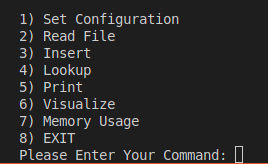
\includegraphics[width=0.45\textwidth]{Images/img4.png}
	\caption{Test of Model 2}
	\label{fig:Test of Model 2}
\end{figure}



\subsection{Model 3}
If our model is as shown in the following figure:

\begin{figure}[h]
	\centering
	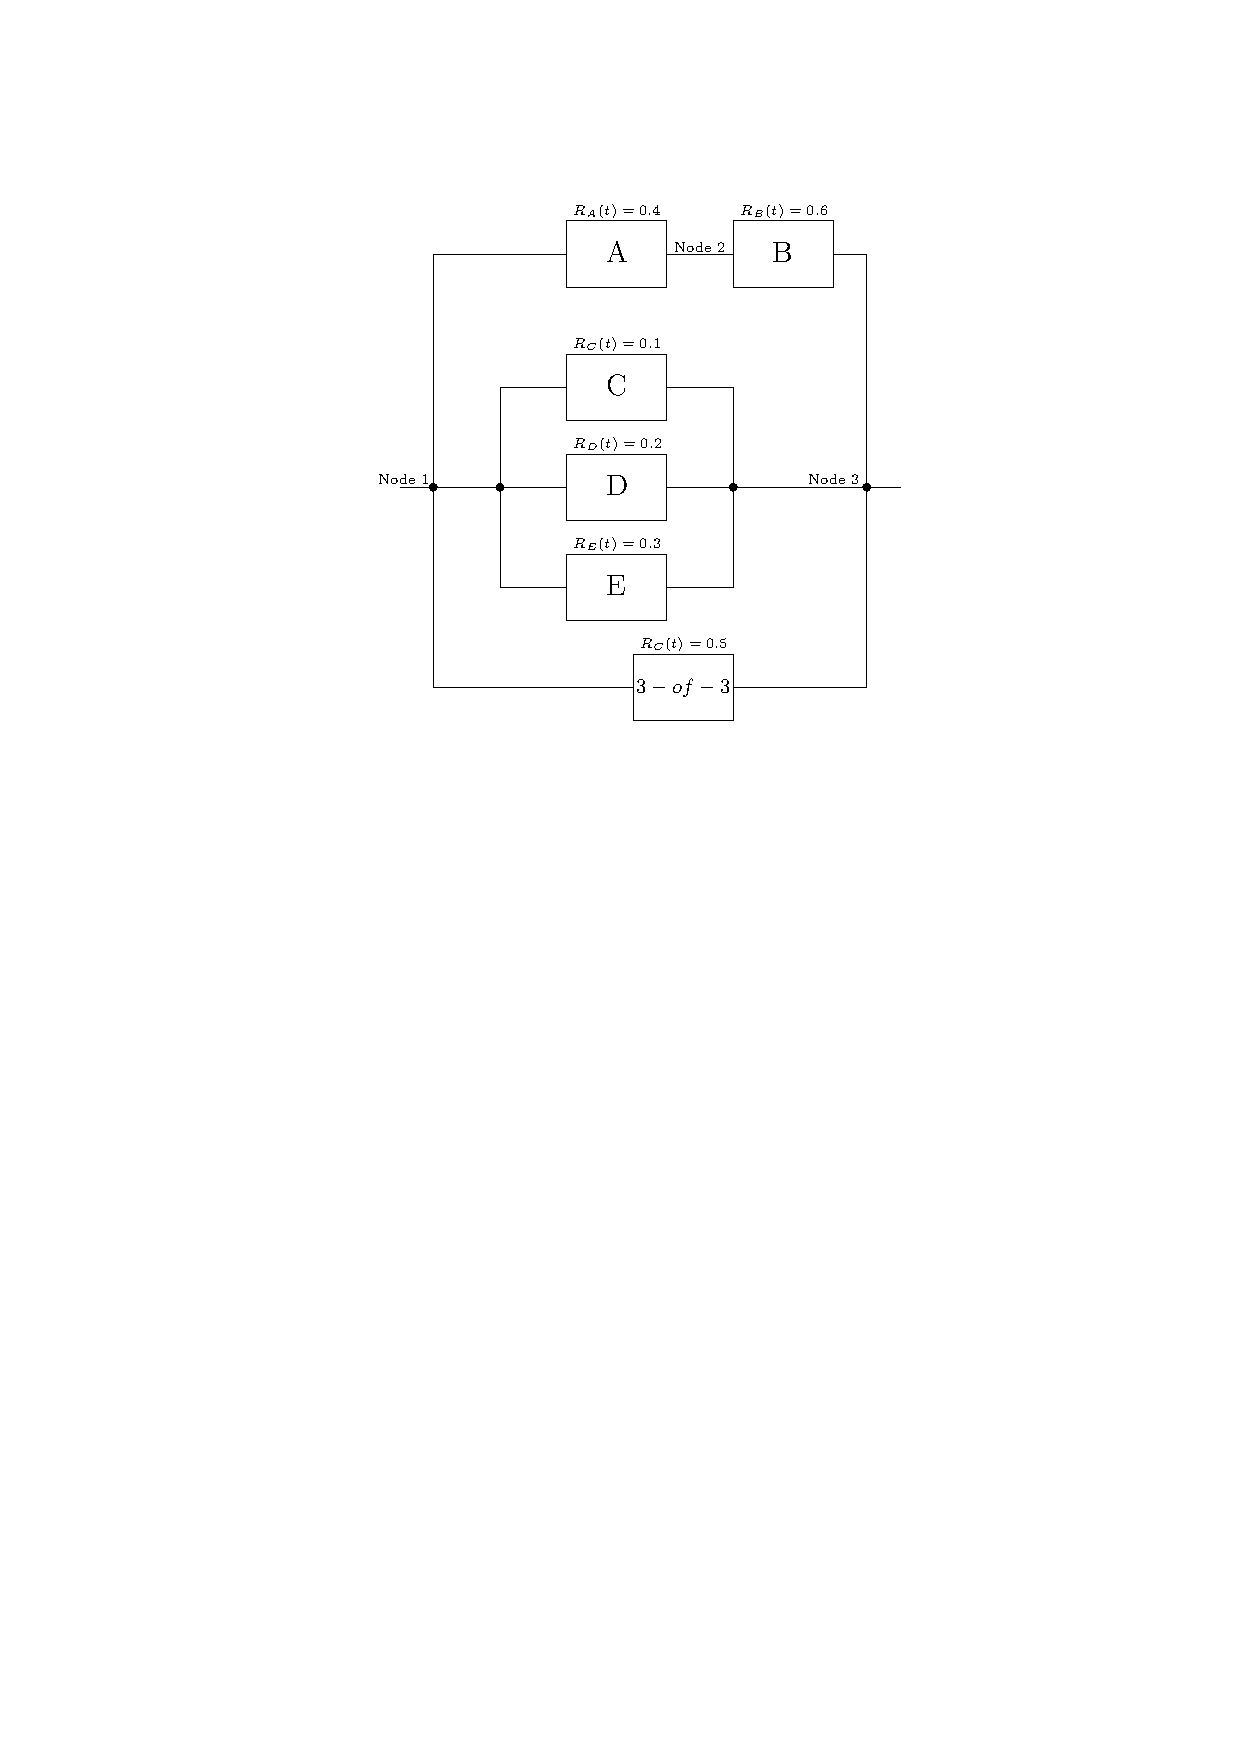
\includegraphics[width=0.4\textwidth]{Images/img4.pdf}
	\caption{Model 3}
	\label{fig:Model 3}
\end{figure}

It can be theoretically solved as follows:

\paragraph{Problem Setup}
We are given the following subsystems:
\begin{itemize}
	\item $A-1-2-0.4$: Subsystem $A$ connects node 1 to node 2 with reliability $0.4$.
	\item $B-2-3-0.6$: Subsystem $B$ connects node 2 to node 3 with reliability $0.6$.
	\item $C-1-3-0.1$: Subsystem $C$ connects node 1 to node 3 with reliability $0.1$.
	\item $D-1-3-0.2$: Subsystem $D$ connects node 1 to node 3 with reliability $0.2$.
	\item $E-1-3-0.3$: Subsystem $E$ connects node 1 to node 3 with reliability $0.3$.
	\item $3\text{of}3-1-3-0.5$: A $3$-of-$3$ subsystem connects node 1 to node 3 with reliability $0.5$.
\end{itemize}

The system configuration is as follows:
\begin{itemize}
	\item Subsystems $A$ and $B$ form a \textbf{series} path from node $1 \to 2 \to 3$.
	\item Subsystems $C$, $D$, $E$, and the $3$-of-$3$ subsystem are in \textbf{parallel} with the series combination of $A+B$.
\end{itemize}

\paragraph{Step 1: Series Combination of $A$ and $B$}
For the series combination of $A$ and $B$, the reliability is:
\[
R_{\text{series}} = R_A \cdot R_B
\]
Substituting $R_A = 0.4$ and $R_B = 0.6$:
\[
R_{\text{series}} = 0.4 \cdot 0.6 = 0.24
\]

\paragraph{Step 2: Reliability of the $3$-of-$3$ Subsystem}
The reliability of a $3$-of-$3$ subsystem is calculated as:
\[
R_{3\text{-of-}3} = \sum_{i=3}^3 \binom{3}{i} R^i (1 - R)^{3-i}
\]
Substituting $R = 0.5$:
\[
R_{3\text{-of-}3} = \binom{3}{3} R^3 (1 - R)^0
\]
\[
R_{3\text{-of-}3} = 1 \cdot (0.5)^3 \cdot 1 = 0.125
\]

\paragraph{Step 3: Parallel Combination of All Paths}
The components in parallel are:
\begin{itemize}
	\item $R_{\text{series}} = 0.24$ (from $A + B$),
	\item $R_C = 0.1$,
	\item $R_D = 0.2$,
	\item $R_E = 0.3$,
	\item $R_{3\text{-of-}3} = 0.125$.
\end{itemize}
The reliability of the parallel combination is given by:
\[
R_{\text{parallel}} = 1 - \prod_{i=1}^n (1 - R_i)
\]
Substituting the values:
\[
R_{\text{parallel}} = 1 - \left[(1 - 0.24) \cdot (1 - 0.1) \cdot (1 - 0.2) \cdot (1 - 0.3) \cdot (1 - 0.125)\right]
\]
Calculate each term:
\[
(1 - 0.24) = 0.76, \quad (1 - 0.1) = 0.9, \quad (1 - 0.2) = 0.8, \quad (1 - 0.3) = 0.7, \quad (1 - 0.125) = 0.875
\]
\[
R_{\text{parallel}} = 1 - \left[0.76 \cdot 0.9 \cdot 0.8 \cdot 0.7 \cdot 0.875\right]
\]
Compute step by step:
\[
0.76 \cdot 0.9 = 0.684, \quad 0.684 \cdot 0.8 = 0.5472, \quad 0.5472 \cdot 0.7 = 0.38304, \quad 0.38304 \cdot 0.875 = 0.33516
\]
\[
R_{\text{parallel}} = 1 - 0.33516 = 0.66484
\]

\paragraph{Final Answer}
The total reliability of the system is approximately:
\[
\boxed{0.665}
\]


If we provide the same input to the application, the output will match the results of our analysis.

\begin{figure}[h]
	\centering
	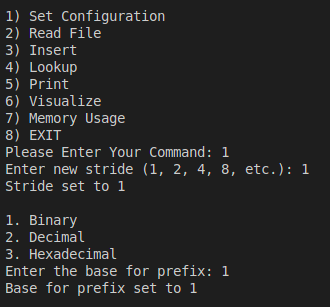
\includegraphics[width=0.45\textwidth]{Images/img5.png}
	\caption{Test of Model 3}
	\label{fig:Test of Model 3}
\end{figure}

\newpage


\subsection{Model 4}
If our model is as shown in the following figure:

\begin{figure}[h]
	\centering
	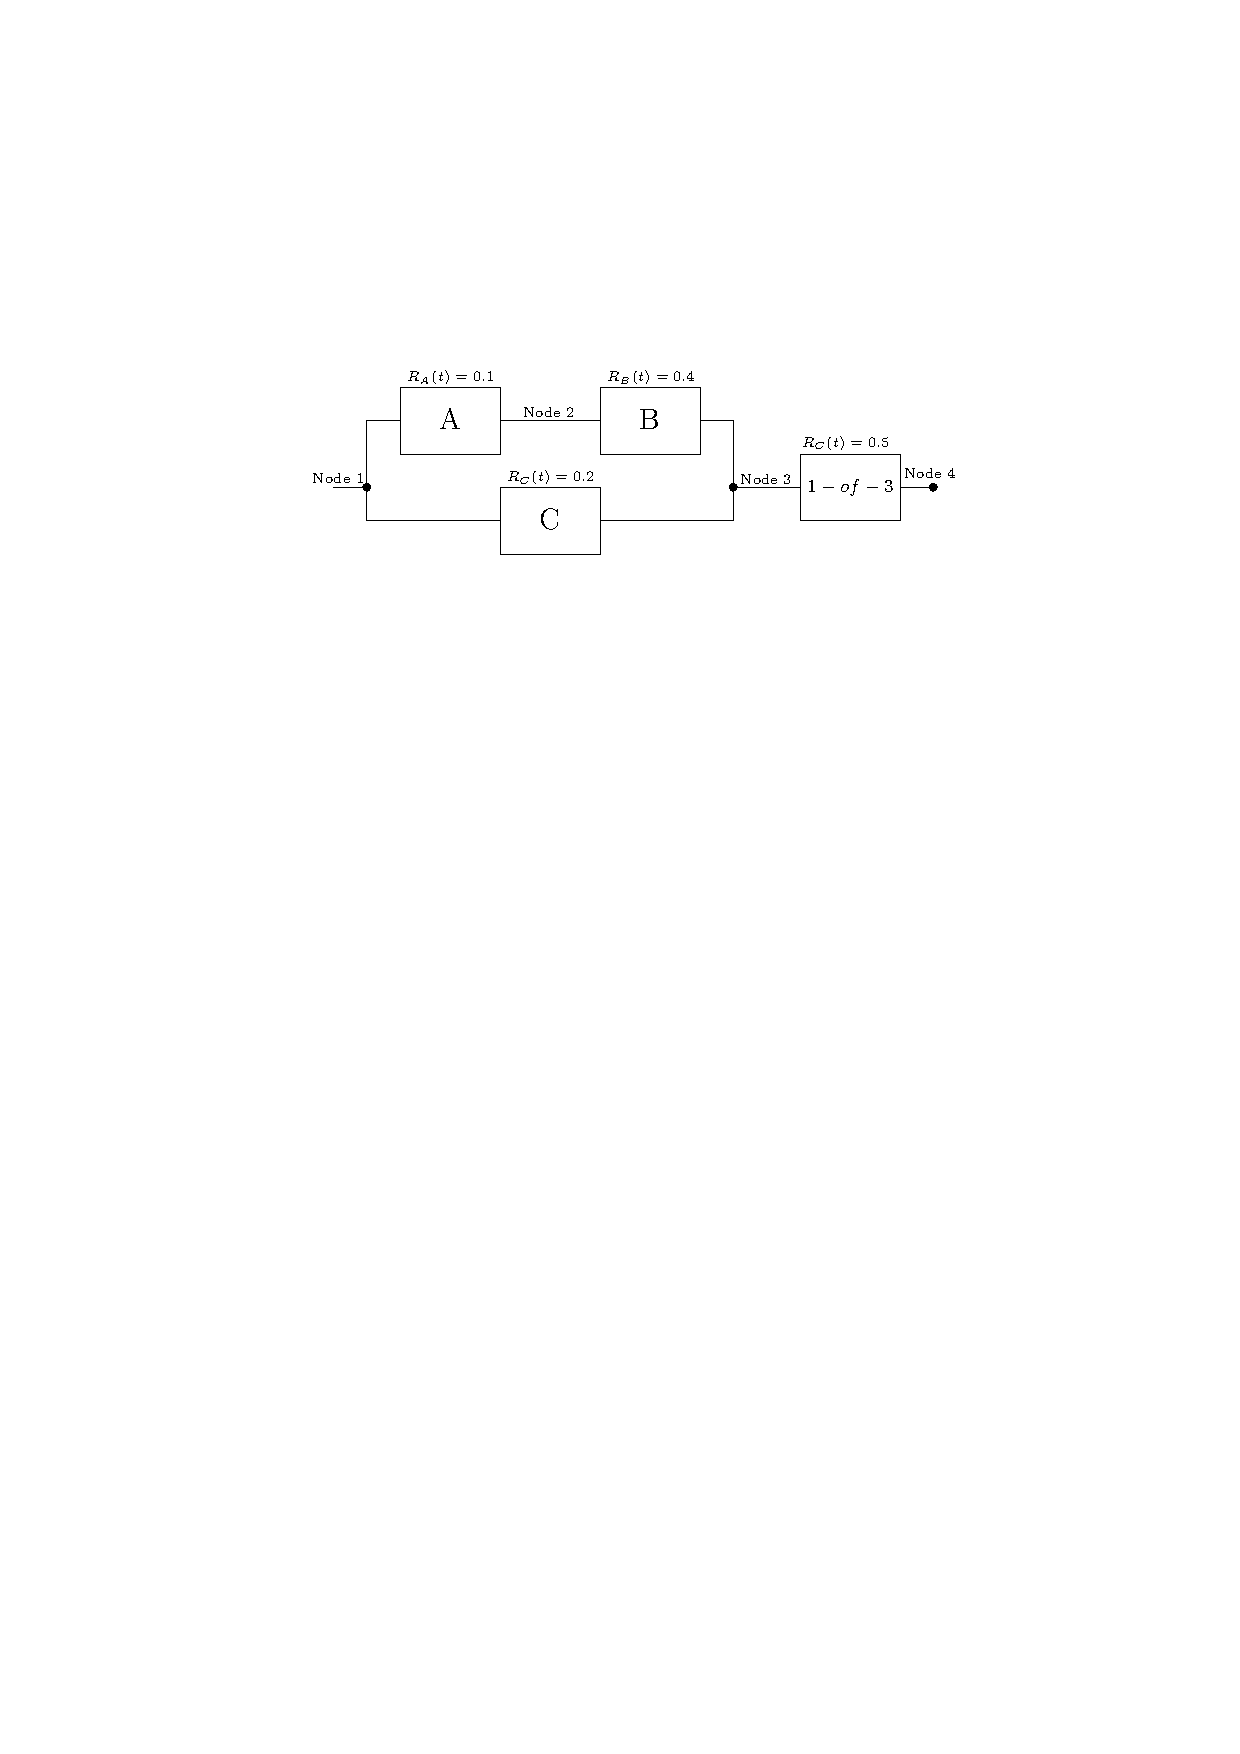
\includegraphics[width=0.65\textwidth]{Images/img5.pdf}
	\caption{Model 4}
	\label{fig:Model 4}
\end{figure}

It can be theoretically solved as follows:


\paragraph{Problem Setup}
We are given the following subsystems:
\begin{itemize}
	\item $A-1-2-0.1$: Subsystem $A$ connects node $1$ to node $2$ with reliability $0.1$.
	\item $B-2-3-0.4$: Subsystem $B$ connects node $2$ to node $3$ with reliability $0.4$.
	\item $C-1-3-0.2$: Subsystem $C$ connects node $1$ to node $3$ with reliability $0.2$.
	\item $1\text{of}3-3-4-0.5$: A $1$-of-$3$ subsystem connects node $3$ to node $4$ with reliability $0.5$.
\end{itemize}

The system configuration is as follows:
\begin{itemize}
	\item Subsystems $A$ and $B$ are in \textbf{series}, forming a path from node $1 \to 2 \to 3$.
	\item Subsystem $C$ is in \textbf{parallel} with the $A+B$ path, connecting nodes $1 \to 3$.
	\item The $1$-of-$3$ subsystem connects node $3$ to node $4$.
\end{itemize}

\paragraph{Step 1: Series Combination of $A$ and $B$}
For the series combination of $A$ and $B$, the reliability is:
\[
R_{\text{series}} = R_A \cdot R_B
\]
Substituting $R_A = 0.1$ and $R_B = 0.4$:
\[
R_{\text{series}} = 0.1 \cdot 0.4 = 0.04
\]

\paragraph{Step 2: Parallel Combination of $R_{\text{series}}$ and $C$}
For the parallel combination of the $A+B$ series ($R_{\text{series}} = 0.04$) and $C$ ($R_C = 0.2$), the reliability is:
\[
R_{\text{parallel}} = 1 - \left[(1 - R_{\text{series}}) \cdot (1 - R_C)\right]
\]
Substituting:
\[
R_{\text{parallel}} = 1 - \left[(1 - 0.04) \cdot (1 - 0.2)\right]
\]
\[
R_{\text{parallel}} = 1 - \left[0.96 \cdot 0.8\right]
\]
\[
R_{\text{parallel}} = 1 - 0.768 = 0.232
\]

\paragraph{Step 3: $1$-of-$3$ Subsystem}
The reliability of a $1$-of-$3$ subsystem is calculated as:
\[
R_{1\text{-of-}3} = \sum_{i=1}^3 \binom{3}{i} R^i (1 - R)^{3-i}
\]
Substituting $R = 0.5$:
\[
R_{1\text{-of-}3} = \binom{3}{1} R^1 (1 - R)^2 + \binom{3}{2} R^2 (1 - R)^1 + \binom{3}{3} R^3 (1 - R)^0
\]
Calculate each term:
\begin{itemize}
	\item For $i = 1$:
	\[
	\binom{3}{1} R^1 (1 - R)^2 = 3 \cdot (0.5)^1 \cdot (0.5)^2 = 3 \cdot 0.5 \cdot 0.25 = 0.375
	\]
	\item For $i = 2$:
	\[
	\binom{3}{2} R^2 (1 - R)^1 = 3 \cdot (0.5)^2 \cdot (0.5)^1 = 3 \cdot 0.25 \cdot 0.5 = 0.375
	\]
	\item For $i = 3$:
	\[
	\binom{3}{3} R^3 (1 - R)^0 = 1 \cdot (0.5)^3 \cdot 1 = 0.125
	\]
\end{itemize}
Summing these:
\[
R_{1\text{-of-}3} = 0.375 + 0.375 + 0.125 = 0.875
\]

\paragraph{Step 4: Series Combination of $R_{\text{parallel}}$ and $R_{1\text{-of-}3}$}
The combined reliability of $R_{\text{parallel}}$ and $R_{1\text{-of-}3}$ in series is:
\[
R_{\text{total}} = R_{\text{parallel}} \cdot R_{1\text{-of-}3}
\]
Substituting $R_{\text{parallel}} = 0.232$ and $R_{1\text{-of-}3} = 0.875$:
\[
R_{\text{total}} = 0.232 \cdot 0.875 = 0.203
\]

\paragraph{Step 5: Final Answer}
The total reliability of the system is approximately:
\[
\boxed{0.203}
\]

If we provide the same input to the application, the output will match the results of our analysis.
\newpage

\begin{figure}[h]
	\centering
	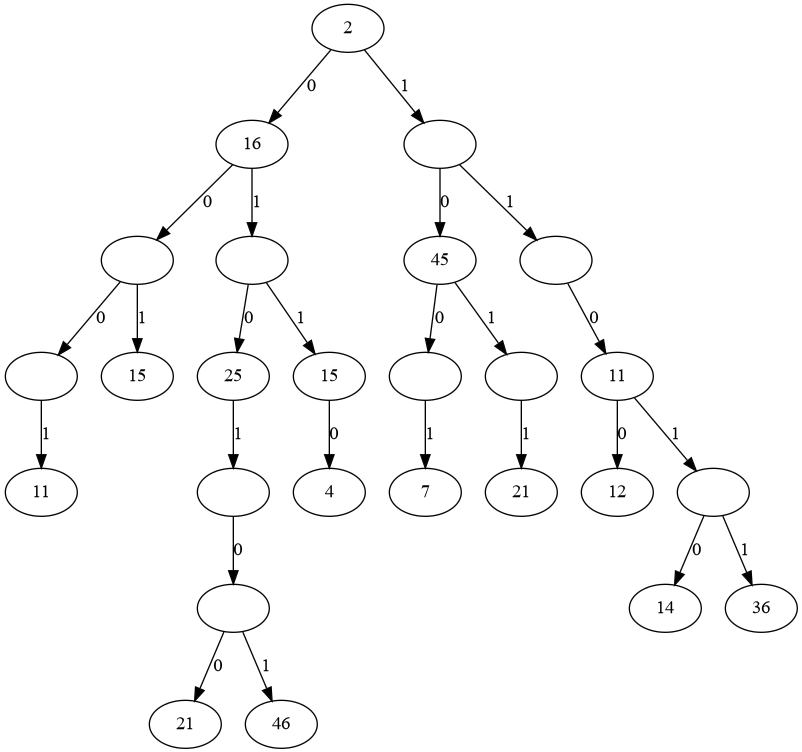
\includegraphics[width=0.45\textwidth]{Images/img6.png}
	\caption{Test of Model 4}
	\label{fig:Test of Model 4}
\end{figure}



\subsection{Model 5}
If our model is as shown in the following figure:

\begin{figure}[h]
	\centering
	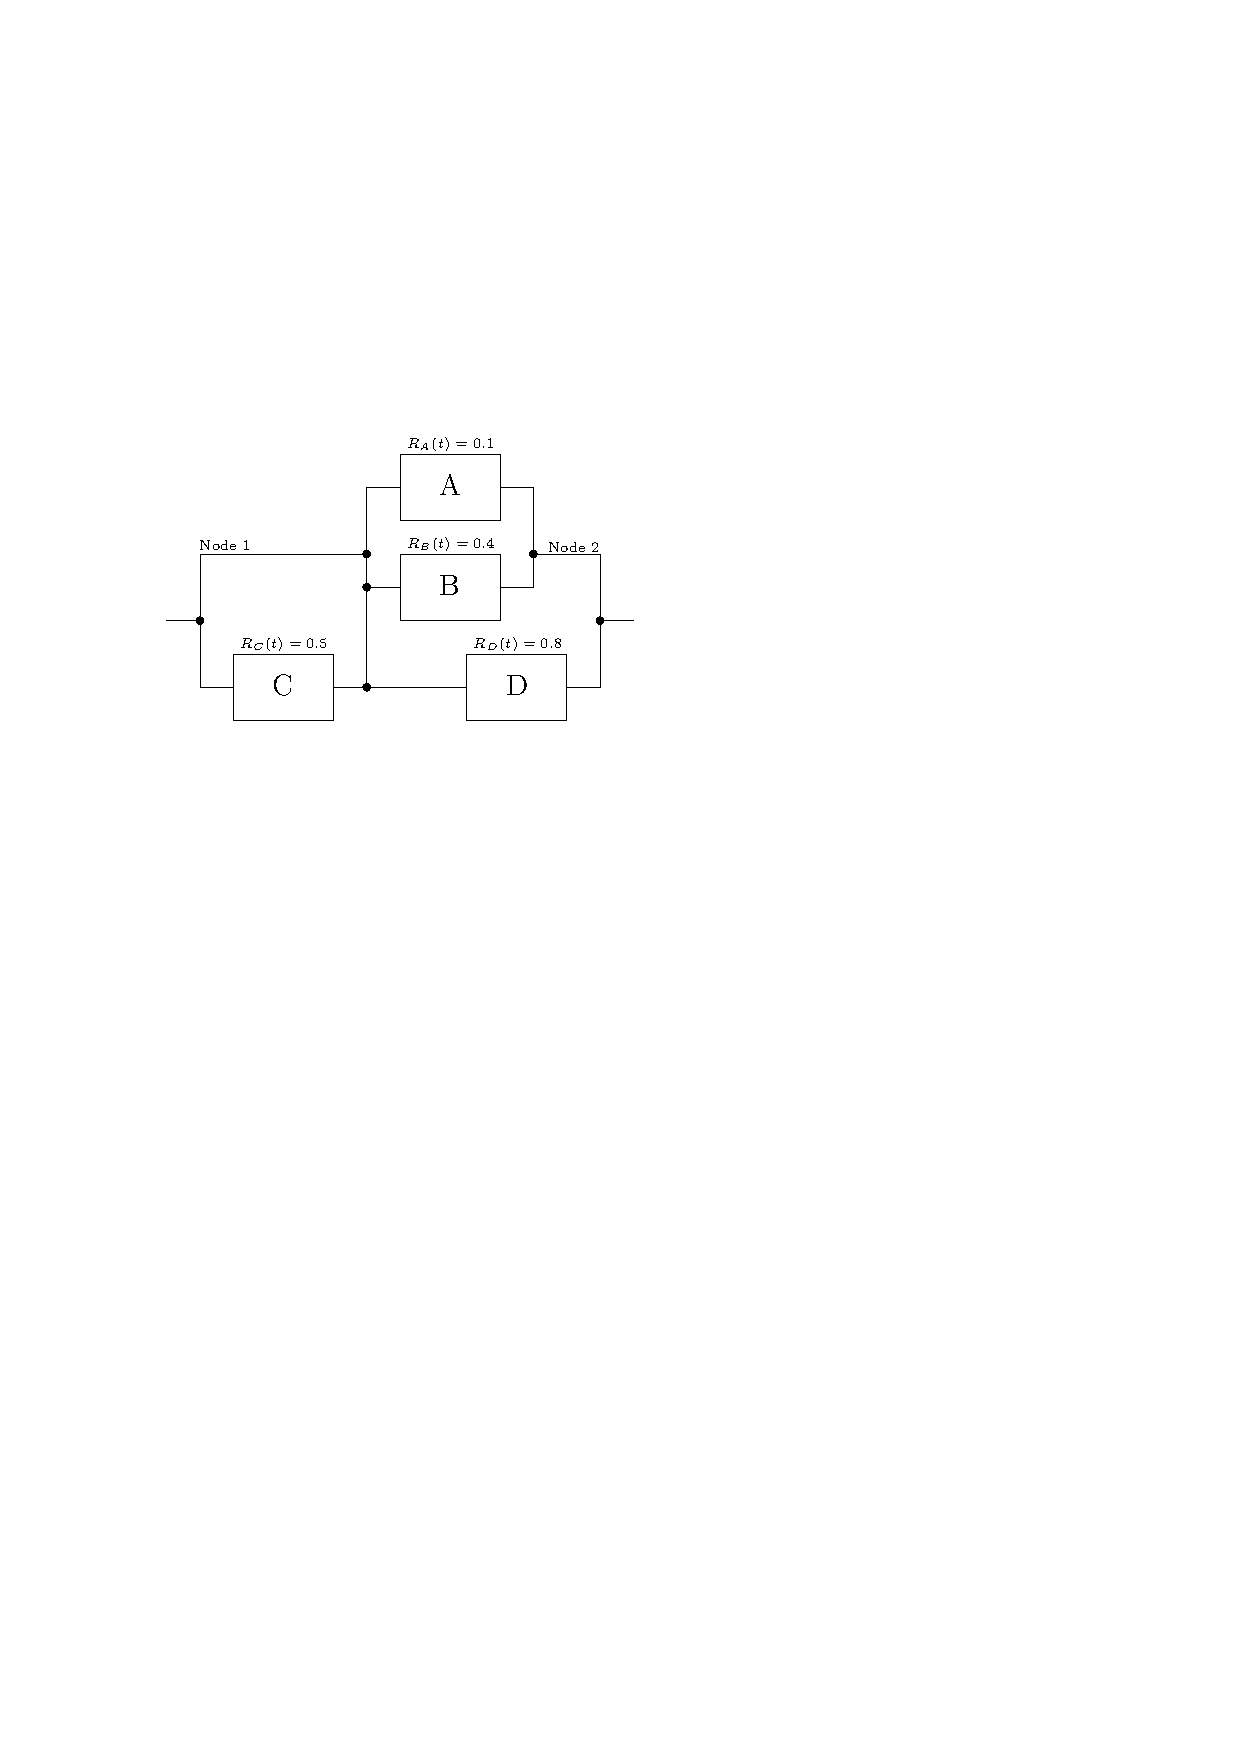
\includegraphics[width=0.65\textwidth]{Images/img6.pdf}
	\caption{Model 5}
	\label{fig:Model 5}
\end{figure}

It can be theoretically solved as follows:

\paragraph{Problem Setup}
We are given the following subsystems:
\begin{itemize}
	\item $A-1-2-0.1$: Subsystem $A$ connects node $1$ to node $2$ with reliability $0.1$.
	\item $B-1-2-0.4$: Subsystem $B$ connects node $1$ to node $2$ with reliability $0.4$.
	\item $C-1-1-0.5$: Subsystem $C$ forms a self-loop at node $1$ with reliability $0.5$.
	\item $D-1-2-0.8$: Subsystem $D$ connects node $1$ to node $2$ with reliability $0.8$.
\end{itemize}

The system configuration is as follows:
\begin{itemize}
	\item Subsystems $A$, $B$, and $D$ are in \textbf{parallel} as they all connect node $1$ to node $2$.
	\item Subsystem $C$ is a \textbf{self-loop} at node $1$, which does not contribute to the reliability between nodes $1$ and $2$.
\end{itemize}

\paragraph{Step 1: Parallel Combination of $A$, $B$, and $D$}
The reliability of parallel subsystems is calculated as:
\[
R_{\text{parallel}} = 1 - \prod_{i=1}^n \left(1 - R_i\right)
\]
Here, the components are $R_A = 0.1$, $R_B = 0.4$, and $R_D = 0.8$. Substituting these values:
\[
R_{\text{parallel}} = 1 - \left[(1 - 0.1) \cdot (1 - 0.4) \cdot (1 - 0.8)\right]
\]
Calculate each term:
\[
(1 - 0.1) = 0.9, \quad (1 - 0.4) = 0.6, \quad (1 - 0.8) = 0.2
\]
\[
R_{\text{parallel}} = 1 - \left[0.9 \cdot 0.6 \cdot 0.2\right]
\]
\[
R_{\text{parallel}} = 1 - (0.9 \cdot 0.6 = 0.54, \quad 0.54 \cdot 0.2 = 0.108)
\]
\[
R_{\text{parallel}} = 1 - 0.108 = 0.892
\]

\paragraph{Step 2: Contribution of Subsystem $C$ (Self-Loop)}
Subsystem $C$ is a self-loop at node $1$. Since it does not contribute to the path between nodes $1$ and $2$, it does not affect the total reliability.

\paragraph{Step 3: Final Answer}
The total reliability of the system is approximately:
\[
\boxed{0.892}
\]

If we provide the same input to the application, the output will match the results of our analysis.
\newpage

\begin{figure}[h]
	\centering
	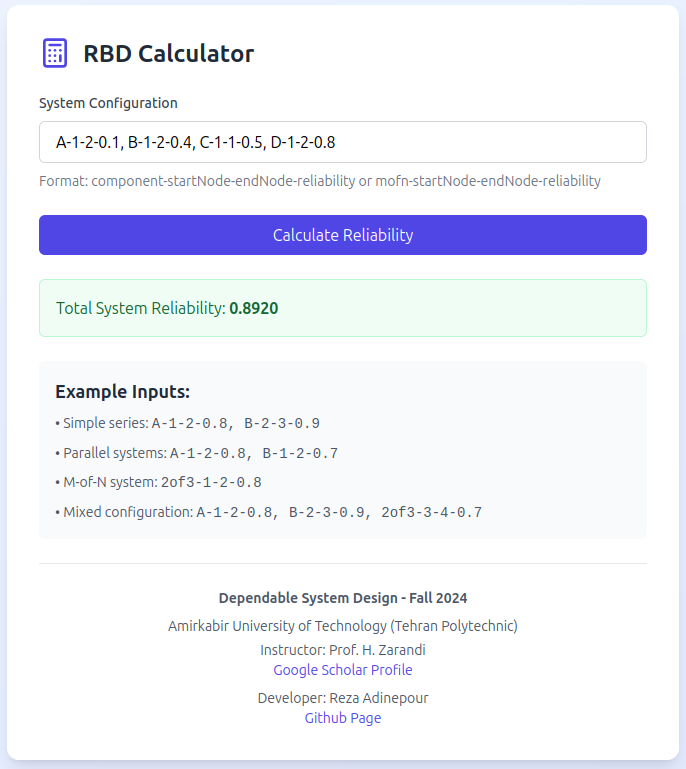
\includegraphics[width=0.45\textwidth]{Images/img7.png}
	\caption{Test of Model 5}
	\label{fig:Test of Model 5}
\end{figure}



\section{Codes}
You can find all of codes \href{https://github.com/M-Sc-AUT/M.Sc-Computer-Architecture/tree/main/Dependable%20System%20Design/Project/Project1}{Here}.

\newpage
% ----------------------------------------------------------------------
% References
% ----------------------------------------------------------------------
 \bibliographystyle{plain}
 \bibliography{refs}

\end{document}